\documentclass[../../../main.tex]{subfiles}
\begin{document}

%%%%%%%%%%%%%%%%%%%%%%%%%%%%%%%%%%%%%%%%%
%%%%%%%%%%%%%%%%%%%%%%%%%%%%%%%%%%%%%%%%%
%%%%%%%%%%%%%%%%%%%%%%%%%%%%%%%%%%%%%%%%%
\chapter{Sampling distributions}

We have spoken so for about distributions of an entire population. We can take a sample of a population, and calculate the same statistic for that sample. We can take sample after sample, and collect the computed statistic for each sample. This new collection is called a sampling distribution. A \vocab{sampling distribution} is a collection of the statistics of \emph{samples}. 


%%%%%%%%%%%%%%%%%%%%%%%%%%%%%%%%%%%%%%%%%
%%%%%%%%%%%%%%%%%%%%%%%%%%%%%%%%%%%%%%%%%
\section{How to build a sampling distribution}


%%%%%%%%%%%%%%%%%%%%%%%%%%%%%%%%%%%%%%%%%
\subsection{A population}

Suppose we have some population. For example, the outcomes of a six sided die: 1, 2, 3, 4, 5, and 6. This is our population. 

Each outcome has a probability of $\frac{1}{6}$, so the probability of this population is distributed uniformly across six, discrete outcomes. We can see this in the plot:

\begin{center}
  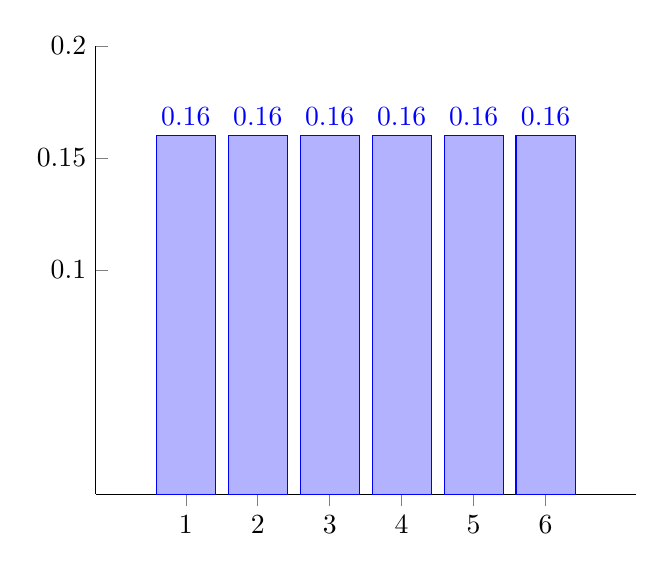
\begin{tikzpicture}
    \begin{axis} [
      axis lines*=left,
      symbolic x coords={1, 2, 3, 4, 5, 6},
      ybar,
      xtick=data,
      ytick={0.1, 0.15, 0.2},
      ymin=0,
      enlarge y limits={value=0.25,upper},
      enlarge x limits=0.25,
      nodes near coords,
      bar width=0.75cm
      ]
      \addplot coordinates {(1, 0.16) (2, 0.16) (3, 0.16) (4, 0.16) (5, 0.16) (6, 0.16)};
    \end{axis}
  \end{tikzpicture}
\end{center}

\noindent
We can calculate the mean for this distribution. We can do that simply by adding up the outcomes and dividing by the number of outcomes:

\begin{equation*}
  \populationmean = \frac{\sum\limits_{i=1}^{\popnum} i}{\popnum} = \frac{1 + 2 + 3 + 4 + 5 + 6}{6} = 3.5
\end{equation*}

\noindent
We can compute the variance too. We do that by computing the average (mean) of the squared deviations:

\begin{equation*}
  \sigma^{2} = \frac{\sum\limits_{i=1}^{n} d^{2}_{i} }{N} = \frac{-2.5^{2} + -1.5^{2} + -0.5^{2} + 0.5^{2} + 1.5^{2} + 2.5^{2}}{6} = 2.92
\end{equation*}

\noindent
And the standard deviation is the square root of that:

\begin{equation*}
  \populationstdev = \sqrt{\sigma^{2}} = \sqrt{2.92} = 1.7
\end{equation*}

\noindent
So we have a population, which has a distribution. It has a mean, and a standard deviation.


%%%%%%%%%%%%%%%%%%%%%%%%%%%%%%%%%%%%%%%%%
\subsection{A sample}

Now, let's take a sample. The first thing we need to do is fix a sample size (which we'll call $\samplesize/$). Let's say that we want a sample of 4 (so $\samplesize/ = 4$. 

Now that we've decided on a sample size, let's randomly select 4 outcomes from the six, and let's call this sample $s_{1}$ (short for ``sample 1''). Suppose we get this sample:

\begin{equation*}
  s_{1} = \{ 1, 4, 5, 3 \}
\end{equation*}

\noindent
We can compute the mean of this sample:

\begin{equation*}
  \frac{1 + 4 + 5. 3}{4} = 3.25
\end{equation*}

\noindent
We call this a \vocab{sample mean}, because it is the mean of a sample. Let's symbolize the mean of the sample as $\SamplingMean/$. So: 

\begin{equation*}
  \SamplingMean/ = \frac{1 + 4 + 5. 3}{4} = 3.25
\end{equation*}

\noindent
Let's put this into a table:

\begin{center}
  \begin{tabular}{| c | c |}
    \hline
    \textbf{Sample} & \textbf{Mean} \\ \hline
    $s_{1}$ & 3.25 \\ \hline
  \end{tabular}
\end{center}

\noindent
What we have just done is taken a sample from our original population, and computed the mean of that sample. Then, we put it into a table.


%%%%%%%%%%%%%%%%%%%%%%%%%%%%%%%%%%%%%%%%%
\subsection{Another sample}

Let's do it again. Let's randomly select 4 outcomes again, for our second sample:

\begin{equation*}
  s_{2} = \{ 2, 2, 3, 1 \}
\end{equation*}

\noindent
We can compute the mean of this sample:

\begin{equation*}
  \SamplingMean/ = \frac{2 + 2 + 3 + 1}{4} = 2.0
\end{equation*}

\noindent
Let's put this into a table:

\begin{center}
  \begin{tabular}{| c | c |}
    \hline
    \textbf{Sample} & \textbf{Mean} \\ \hline
    $s_{1}$ & 3.25 \\ \hline
    $s_{2}$ & 2.0 \\ \hline
  \end{tabular}
\end{center}


%%%%%%%%%%%%%%%%%%%%%%%%%%%%%%%%%%%%%%%%%
\subsection{More and more samples}

Imagine that we repeat this process lots and lots of times. We randomly select 3 outcomes, for each successive sample. For instance:

\begin{multline*}
  s_{3} = \{ 1, 5, 5, 3 \} \\
  s_{4} = \{ 3, 1, 6, 2 \} \\
  s_{5} = \{ 4, 4, 6, 4 \} \\
  s_{6} = \{ 1, 3, 2, 1 \} \\
  s_{7} = \{ 5, 6, 2, 4 \}  
\end{multline*}

\noindent
We compute the means for each new sample, and put them into our table:

\begin{center}
  \begin{tabular}{| c | c |}
    \hline
    \textbf{Sample} & \textbf{Mean} \\ \hline
    $s_{1}$ & 3.25 \\ \hline
    $s_{2}$ & 2.0 \\ \hline
    $s_{3}$ & 3.5 \\ \hline
    $s_{4}$ & 3.0 \\ \hline
    $s_{5}$ & 4.5 \\ \hline
    $s_{6}$ & 1.75 \\ \hline
    $s_{7}$ & 4.25 \\ \hline
  \end{tabular}
\end{center}


%%%%%%%%%%%%%%%%%%%%%%%%%%%%%%%%%%%%%%%%%
\subsection{A sampling distribution}

We have collected a set of sample means. We call them \vocab{sample means} because each one is the mean of a \emph{sample}.

Like any other set of values, this has a distribution. That is, it's values are spread out in some particular way. Let's plot it to see. We'll do it as a histogram:

\begin{center}
  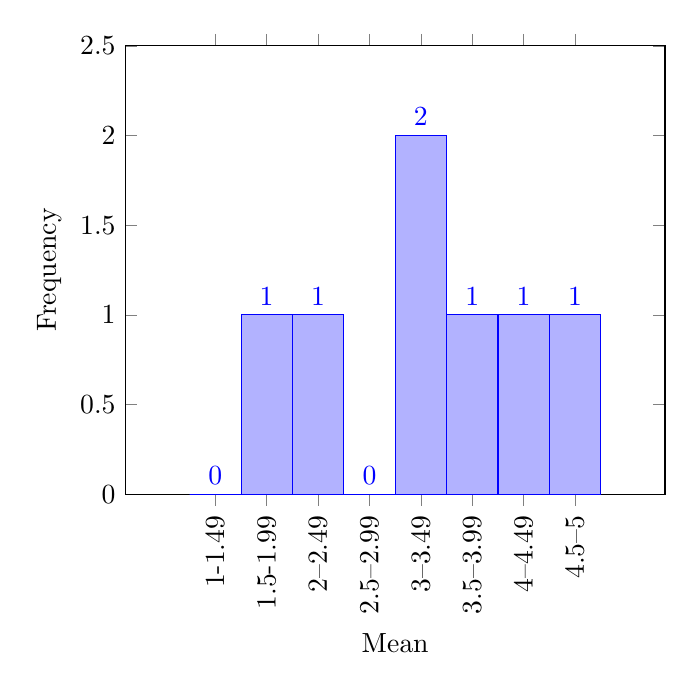
\begin{tikzpicture}
    \begin{axis} [
      ylabel=Frequency,
      xlabel=Mean,
      ybar,
      ymin=0,
      xtick=data,
      xticklabel style={rotate=90},
      symbolic x coords={1-1.49, 1.5-1.99, 2--2.49, 2.5--2.99, 3--3.49, 3.5--3.99, 4--4.49, 4.5--5},
      enlarge y limits={value=0.25,upper},
      enlarge x limits=0.25,
      nodes near coords,
      bar width=0.65cm,
      ]
      \addplot coordinates {
        (1-1.49, 0) (1.5-1.99, 1) (2--2.49, 1) (2.5--2.99, 0) (3--3.49, 2) (3.5--3.99, 1) (4--4.49, 1) (4.5--5, 1)
      };
    \end{axis}
  \end{tikzpicture}
\end{center}


%%%%%%%%%%%%%%%%%%%%%%%%%%%%%%%%%%%%%%%%%
\subsection{More samples}

We can take lots more samples:

\begin{align*}
  s_{8} = \{ 2, 3, 4, 2 \} \hskip 1cm s_{12} = \{ 4, 2, 3, 5 \} \\
  s_{9} = \{ 6, 2, 4, 3 \} \hskip 1cm s_{13} = \{ 4, 2, 3, 3 \} \\
  s_{10} = \{ 1, 2, 6, 2 \} \hskip 1cm s_{14} = \{ 2, 3, 4, 1 \} \\
  s_{11} = \{ 6, 1, 1, 2 \} \hskip 1cm s_{15} = \{ 1, 4, 4, 5 \}
\end{align*}

\noindent
And build up our table of sample means even more:

\begin{center}
  \begin{tabular}{| c | c || c | c |}
    \hline
    \textbf{Sample} & \textbf{Mean} & \textbf{Sample} & \textbf{Mean} \\ \hline
    \ldots & \ldots & \ldots & \ldots \\ \hline
    $s_{8}$ & 2.75 & $s_{12}$ & 4.0 \\ \hline
    $s_{9}$ & 3.75 & $s_{13}$ & 3.0 \\ \hline
    $s_{10}$ & 2.75 & $s_{14}$ & 2.5 \\ \hline
    $s_{11}$ & 2.5 & $s_{15}$ & 3.5 \\ \hline
  \end{tabular}
\end{center}

\noindent
We can add these new values to the plot: 

\begin{center}
  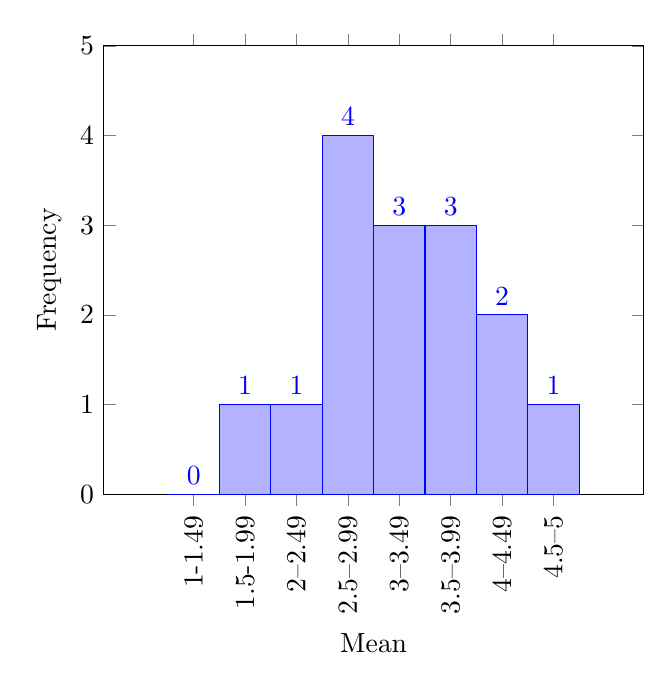
\begin{tikzpicture}
    \begin{axis} [
      ylabel=Frequency,
      xlabel=Mean,
      ybar,
      ymin=0,
      xtick=data,
      xticklabel style={rotate=90},
      symbolic x coords={1-1.49, 1.5-1.99, 2--2.49, 2.5--2.99, 3--3.49, 3.5--3.99, 4--4.49, 4.5--5},
      enlarge y limits={value=0.25,upper},
      enlarge x limits=0.25,
      nodes near coords,
      bar width=0.65cm,
      ]
      \addplot coordinates {
        (1-1.49, 0) (1.5-1.99, 1) (2--2.49, 1) (2.5--2.99, 4) (3--3.49, 3) (3.5--3.99, 3) (4--4.49, 2) (4.5--5, 1)
      };
    \end{axis}
  \end{tikzpicture}
\end{center}


%%%%%%%%%%%%%%%%%%%%%%%%%%%%%%%%%%%%%%%%%
\subsection{Adding more}

We can take even more samples:

\begin{align*}
  s_{16} = \{ 6, 2, 3, 4 \} \hskip 1cm s_{20} = \{ 4, 4, 1, 4 \} \\
  s_{17} = \{ 5, 4, 3, 6 \} \hskip 1cm s_{21} = \{ 4, 5, 2, 5 \} \\
  s_{18} = \{ 5, 3, 3, 1 \} \hskip 1cm s_{22} = \{ 1, 6, 2, 4 \} \\
  s_{19} = \{ 4, 6, 3, 3 \} \hskip 1cm s_{23} = \{ 6, 1, 2, 1 \} 
\end{align*}

\noindent
And build up our collection of sample means even more:

\begin{center}
  \begin{tabular}{| c | c || c | c |}
    \hline
    \textbf{Sample} & \textbf{Mean} & \textbf{Sample} & \textbf{Mean} \\ \hline
    \ldots & \ldots & \ldots & \ldots \\ \hline
    $s_{16}$ & 3.75 & $s_{20}$ & 3.25 \\ \hline
    $s_{17}$ & 4.5 & $s_{21}$ & 4.0 \\ \hline
    $s_{18}$ & 3.0 & $s_{22}$ & 3.25 \\ \hline
    $s_{19}$ & 4.0 & $s_{23}$ & 2.5 \\ \hline
  \end{tabular}
\end{center}

\noindent
And we can add the new values to the plot again: 

\begin{center}
  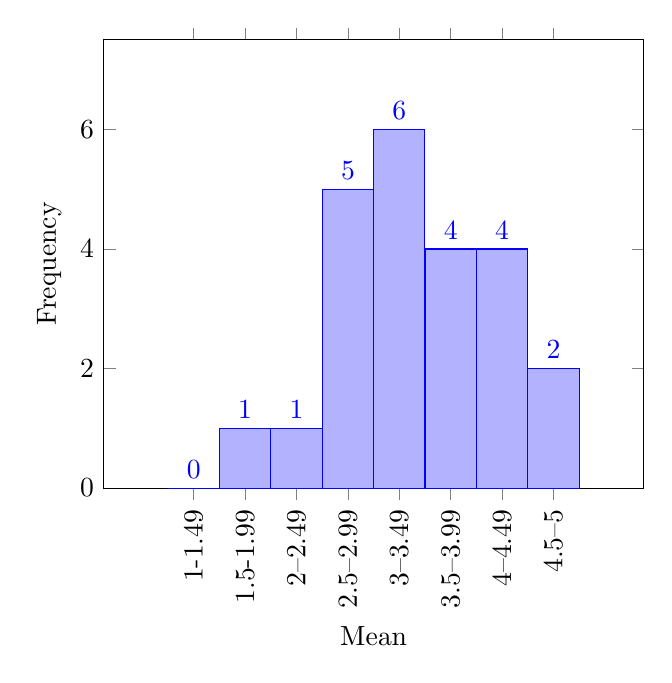
\begin{tikzpicture}
    \begin{axis} [
      ylabel=Frequency,
      xlabel=Mean,
      ybar,
      ymin=0,
      xtick=data,
      xticklabel style={rotate=90},
      symbolic x coords={1-1.49, 1.5-1.99, 2--2.49, 2.5--2.99, 3--3.49, 3.5--3.99, 4--4.49, 4.5--5},
      enlarge y limits={value=0.25,upper},
      enlarge x limits=0.25,
      nodes near coords,
      bar width=0.65cm,
      ]
      \addplot coordinates {
        (1-1.49, 0) (1.5-1.99, 1) (2--2.49, 1) (2.5--2.99, 5) (3--3.49, 6) (3.5--3.99, 4) (4--4.49, 4) (4.5--5, 2)
      };
    \end{axis}
  \end{tikzpicture}
\end{center}


%%%%%%%%%%%%%%%%%%%%%%%%%%%%%%%%%%%%%%%%%
\subsection{One more round}

One more round:

\begin{align*}
  s_{24} = \{ 5, 5, 2, 3 \} \hskip 1cm s_{29} = \{ 5, 3, 3, 4 \} \\
  s_{25} = \{ 5, 5, 3, 5 \} \hskip 1cm s_{30} = \{ 2, 4, 6, 3 \} \\
  s_{26} = \{ 2, 4, 6, 4 \} \hskip 1cm s_{31} = \{ 6, 4, 1, 1 \} \\
  s_{27} = \{ 3, 3, 3, 3 \} \hskip 1cm s_{32} = \{ 3, 3, 2, 1 \} \\
  s_{28} = \{ 4, 1, 1, 2 \} \hskip 1cm s_{33} = \{ 6, 1, 1, 3 \}  
\end{align*}

\noindent
The table:

\begin{center}
  \begin{tabular}{| c | c || c | c |}
    \hline
    \textbf{Sample} & \textbf{Mean} & \textbf{Sample} & \textbf{Mean} \\ \hline
    \ldots & \ldots & \ldots & \ldots \\ \hline
    $s_{24}$ & 3.75 & $s_{29}$ & 3.75 \\ \hline
    $s_{25}$ & 4.5 & $s_{30}$ & 3.75 \\ \hline
    $s_{26}$ & 4.0 & $s_{31}$ & 3.0 \\ \hline
    $s_{27}$ & 3.0 & $s_{32}$ & 2.25 \\ \hline
    $s_{28}$ & 2.0 & $s_{33}$ & 2.75 \\ \hline
  \end{tabular}
\end{center}

\noindent
And the plot:

\begin{center}
  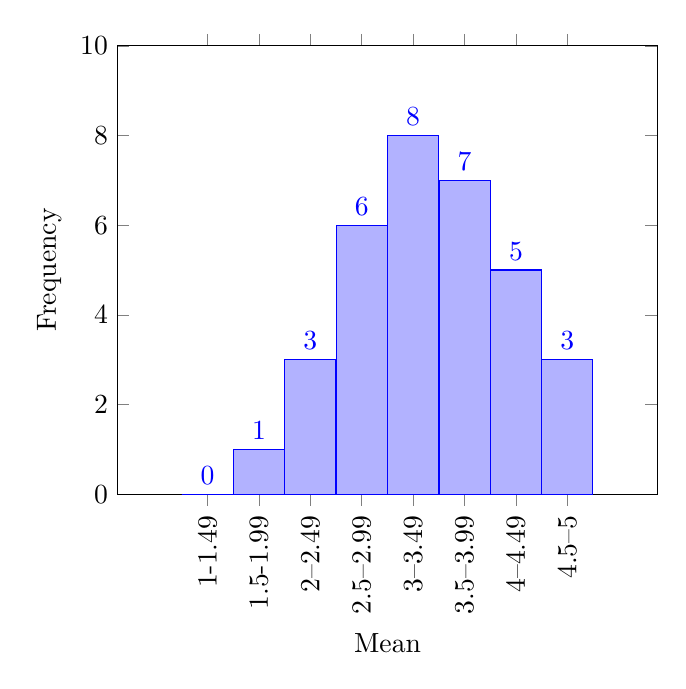
\begin{tikzpicture}
    \begin{axis} [
      ylabel=Frequency,
      xlabel=Mean,
      ybar,
      ymin=0,
      xtick=data,
      xticklabel style={rotate=90},
      symbolic x coords={1-1.49, 1.5-1.99, 2--2.49, 2.5--2.99, 3--3.49, 3.5--3.99, 4--4.49, 4.5--5},
      enlarge y limits={value=0.25,upper},
      enlarge x limits=0.25,
      nodes near coords,
      bar width=0.65cm,
      ]
      \addplot coordinates {
        (1-1.49, 0) (1.5-1.99, 1) (2--2.49, 3) (2.5--2.99, 6) (3--3.49, 8) (3.5--3.99, 7) (4--4.49, 5) (4.5--5, 3)
      };
    \end{axis}
  \end{tikzpicture}
\end{center}


%%%%%%%%%%%%%%%%%%%%%%%%%%%%%%%%%%%%%%%%%
\subsection{Observations}

Take note of the following observations:

\begin{itemize}

  \item We started with a population (the set of outcomes for a six-sided die), and we started taking samples (of size 4) from that population. We computed the mean for each sample, and we dumped each mean into our table. In this way, we built up a collection of sample means. This is a \vocab{sampling distribution}, because it is a collection of statistics that we constructed through sampling.

  \item Even though this is a set of sample means, taken from our original population, it is still just a set of values, like any other data set. So it is a \vocab{distribution}, just like any other data set. And like any other data set, it has a \vocab{mean}, \vocab{variance}, and \vocab{standard deviation}.

  \item Notice the shape of the sampling distribution. As we added more and more sample means, the shape started to look more and more like a \vocab{normal curve}. This is not a coincidence. It turns out that sampling distributions \emph{always} look more and more like normal curves as you build them up more and more, especially when you take large enough samples. 
  
  \item Even though the sampling distribution looks normally distributed, the original population that we took the samples from is \emph{not} normally distributed. On the contrary, the original population is uniformly distributed. It turns out that sampling distributions will still end up with a normal shape, \vocab{regardless of the population's shape} they are sampled from, especially when you take large enough samples.

  \item Also, notice where most of the values are clustering. They are clustering around 3.5. Is that value significant? Yes it is. It is the mean of the \emph{population}. Again, this is no coincidence. It turns out that, as you build up the sampling distribution more and more, the \vocab{mean of a sampling distribution} (which we symbolize as $\SamplingMean/$) tends to get closer and closer to the \vocab{mean of the population} (which we symbolize as $\populationmean$), especially when you take large enough samples.

\end{itemize}


%%%%%%%%%%%%%%%%%%%%%%%%%%%%%%%%%%%%%%%%%
%%%%%%%%%%%%%%%%%%%%%%%%%%%%%%%%%%%%%%%%%
\section{Example 2}

In the last example, we dealt with a very simple discrete distribution. But the same thing can be done for continuous data too. To illustrate that, let's think about another (more realistic) example, which uses continuous values. 

Suppose we want to examine all of the 5" carriage bolts produced by Sanders Bolt Manufacturing. These bolts are supposed to weigh 125g each, but of course, manufacturing is imprecise, and no bolt is ever \emph{exactly} 125g. What we want to know is the mean (average) weight of all the bolts.

Unfortunately, we can't weigh every single bolt that the company produces. There are just too many, and the cost can't be justified.

Instead, we must take a sample. The first step is to fix/decide a sample size $\samplesize/$. Suppose we decide to have a sample size of 40 (so $\samplesize/ = 40$). 

So, we select 40 bolts at random, and weigh each of them. Then we use those 40 weights to calculate the mean (average) weight of that sample. That is, we add up all 40 weights, and divide the sum by 40. This gives us the mean weight of the sample. For example, suppose it comes out to 124.97g. The average weight of the 40 bolts we selected is 124.97g.

What we have just done is taken a sample, and computed the mean of that sample. So, although we are interested in the mean of the population, what we have done is taken a sample, and learned the mean only of that \emph{sample}. We call this mean a \vocab{sample mean}, because it is the mean of a sample.

Suppose that we write down this sample mean in a table. Let us say that this is the sample mean for sample 1, or $s_{1}$ for short. Our table looks like this:

\begin{center}
  \begin{tabular}{| c | c |}
    \hline
    \textbf{Sample} & \textbf{Mean} \\ \hline
    $s_{1}$ & 124.97g \\ \hline
  \end{tabular}
\end{center}

\noindent
Next, suppose we put all 40 bolts back, and we repeat the process. So, we randomly select 40 new bolts, to get sample 2, i.e., $s_{2}$. Again, we weigh all of the specimens in our sample, and we compute the mean for $s_{2}$. We write this sample mean down in our table too:

\begin{center}
  \begin{tabular}{| c | c |}
    \hline
    \textbf{Sample} & \textbf{Mean} \\ \hline
    $s_{1}$ & 124.97g \\ \hline
    $s_{2}$ & 123.23g \\ \hline
  \end{tabular}
\end{center}

\noindent
Suppose we repeat this over and over again, building up a bigger and bigger table:

\begin{center}
  \begin{tabular}{| c | c |}
    \hline
    \textbf{Sample} & \textbf{Mean} \\ \hline
    $s_{1}$ & 124.97g \\ \hline
    $s_{2}$ & 123.23g \\ \hline
    $s_{3}$ & 126.65g \\ \hline
    \ldots & \ldots \\ \hline
    $s_{1000}$ & 125.41g \\ \hline
    $s_{1001}$ & 124.02g \\ \hline
  \end{tabular}
\end{center}

\noindent
What we have done here is gathered a large collection of sample means. And like any other collection of values, this data set is a distribution itself. That is to say, its values are spread out in certain places. So what is the shape of this data, exactly?

We can't plot every point of data exactly, because this is made-up data. But we don't really have to plot an exact graph. Since this is a sampling distribution, constructed from a fairly large sample (40 bolts per sample), we know that the values will be distributed normally. That is to say, the plot will look very much like a normal curve. Something like this:

\begin{center}
  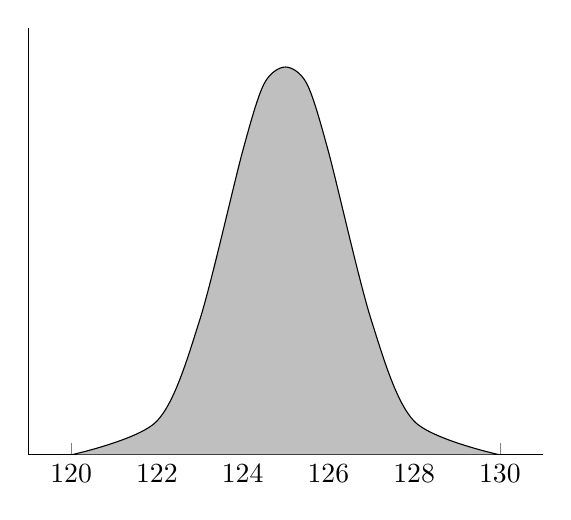
\begin{tikzpicture}
    \begin{axis}[
      axis lines*=left,
      ytick=\empty,
      height=7cm,
      enlarge y limits={value=0.1,upper},
      ]
      \addplot[smooth, fill=lightgray, domain=120:130] 
        coordinates{
          (120, 0) (122, 0.5) (123, 2) (124, 4.5) (124.5, 5.5)
          (125, 5.75)
          (125.5, 5.5) (126, 4.5) (127, 2) (128, 0.5) (130, 0)} 
        \closedcycle;
    \end{axis}
  \end{tikzpicture}
\end{center}

\noindent
Moreover, we know that the values will be clustered around 125g, which is somewhere near the mean of the population we took the samples from. 

If you think about it, this is expected. Most of the bolts weigh close to 125g. Only a few are significantly smaller (like 121g or 122g), and only a few are significantly larger (like 128g or 129g). So we would expect most of the samples to have an average weight that is closer to the mean of the population. Only a few outlier samples would end up including particularly light or particularly heavy bolts.


\end{document}
